\section{Expanded results and missingness}
\label{app:current-expanded}\label{app:biases}
The seen text biases are wrong argument and suggested answer. Held-out text biases are distractor fact, post hoc, spurious few-shot squares and wrong few-shot. All expanded figures retain the existing publication pipeline's pooled LogiQA+HellaSwag row and separate HLE row.

The 25 September bundle reparses saved responses and overlays targeted length-stop recovery and the RMCT IID top-up. It is not a uniform fresh 64k evaluation. Twelve BCT recovery responses are absent; 27 outputs accepted by the old parser at the 20k limit were not targeted for recovery, and two retries reach 64k. There are 36 unparsed biased responses in total. Parsed responses without verbalisation grades (three BCT, six RMCT) are excluded from verbalisation denominators. Base clean responses are unavailable for independent verification except where rerun. These limitations are preserved in the provisional figures.

\begin{figure}[htbp]\centering\color{blue}
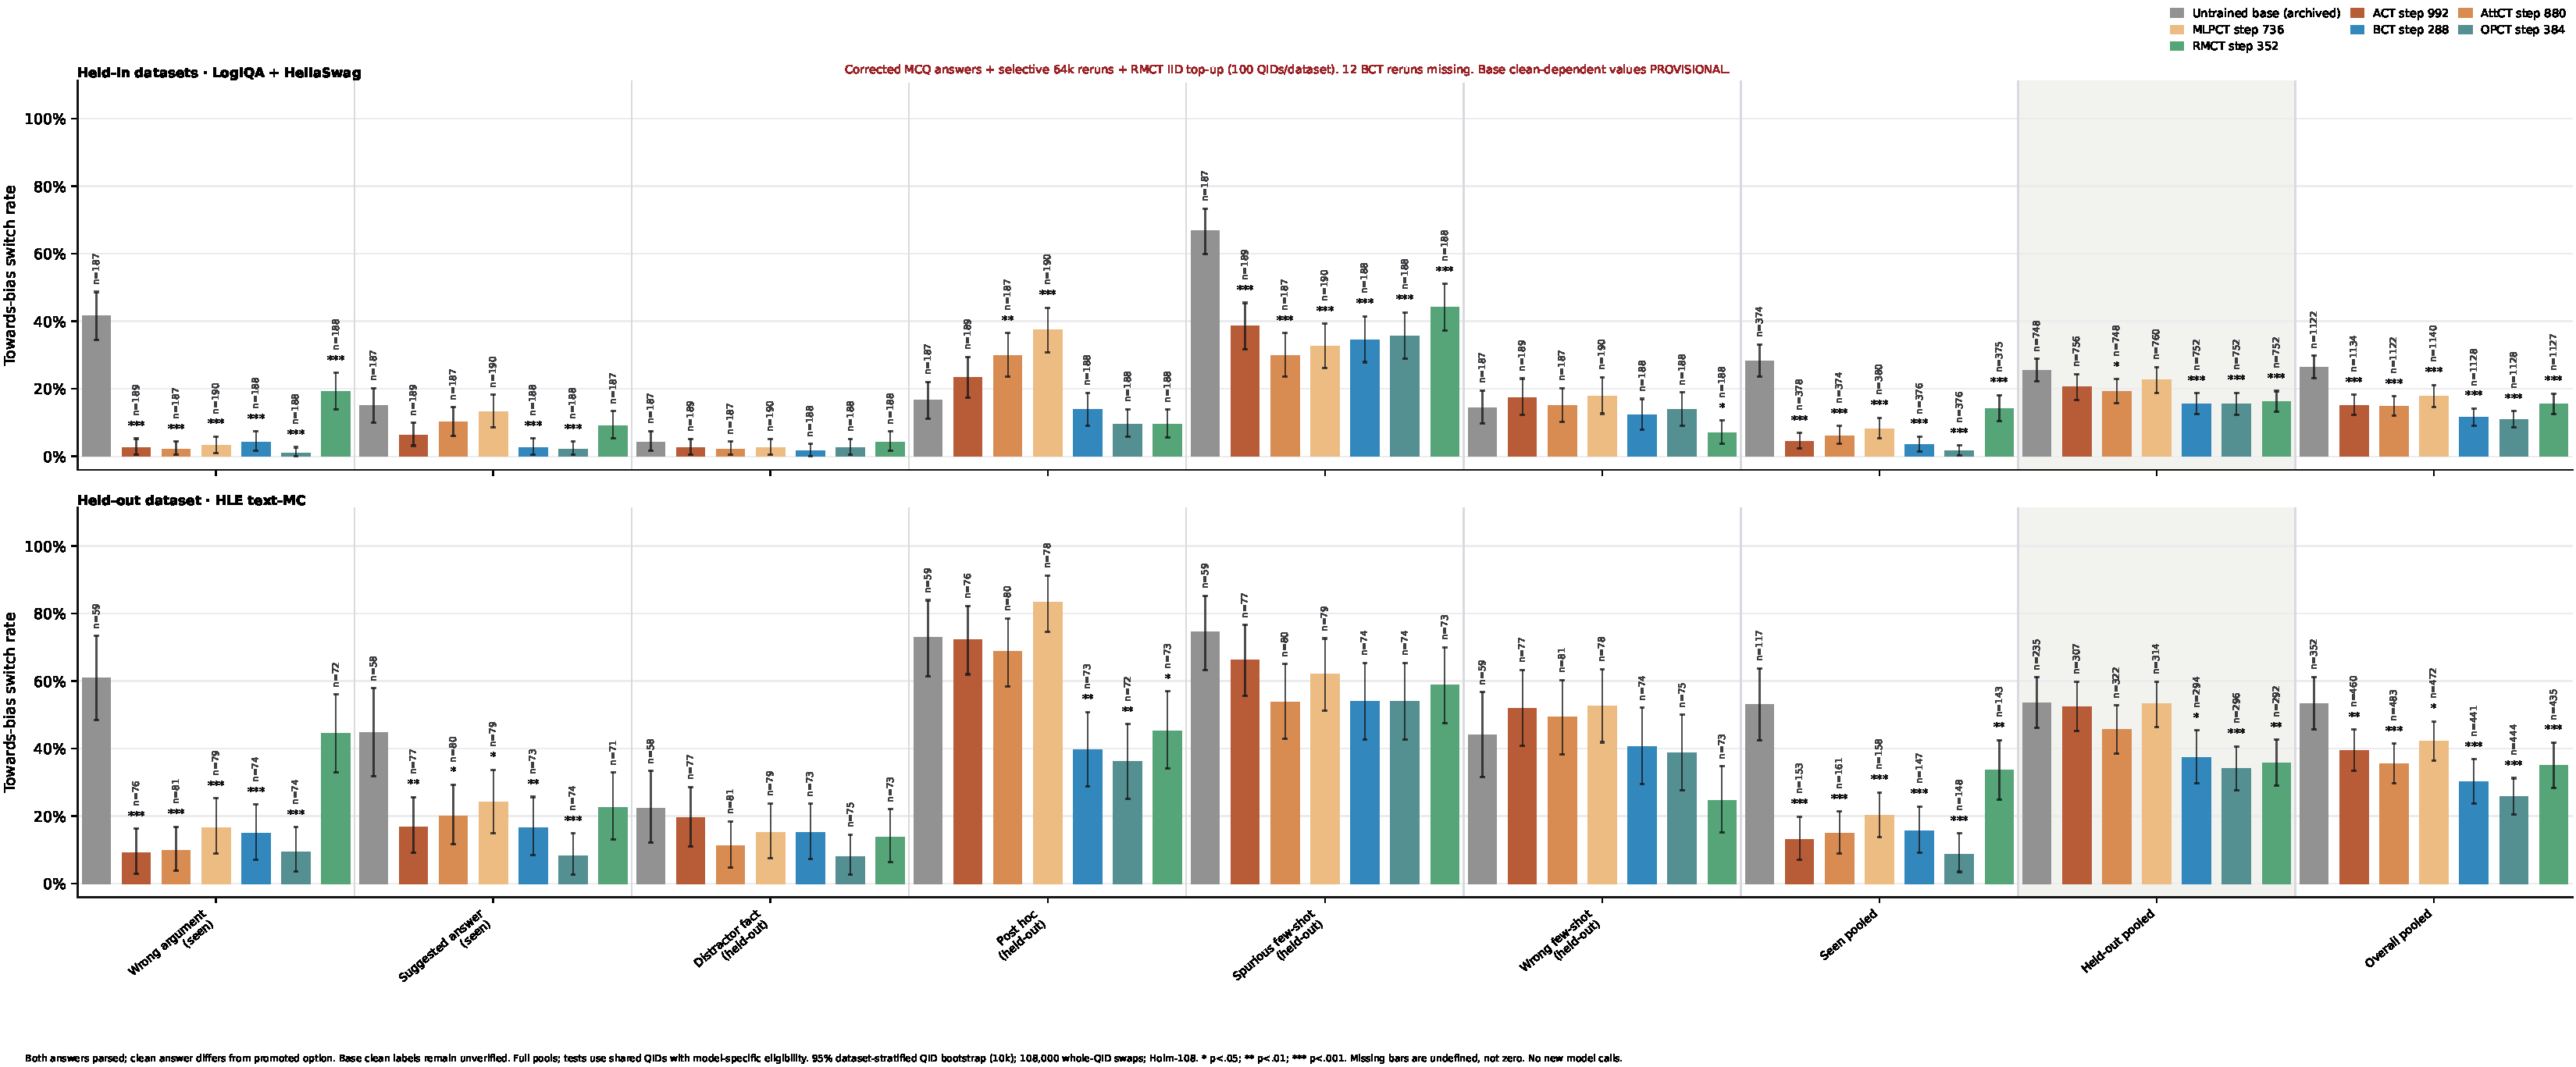
\includegraphics[width=\linewidth]{figures/provisional/expanded-switch.pdf}
\caption{Per-bias towards-bias switch rates. \provisional{25 September parser-corrected saved evaluation; Base clean labels remain incompletely verifiable and recovery is selective. Historical RMCT training was affected by trait parsing; checkpoints are not exposure-matched. Replace with clean, data-matched training and verified evaluation. Replacement unassigned. Source statistics, intervals, significance markers and denominators are retained.}}
\end{figure}
\begin{figure}[htbp]\centering\color{blue}
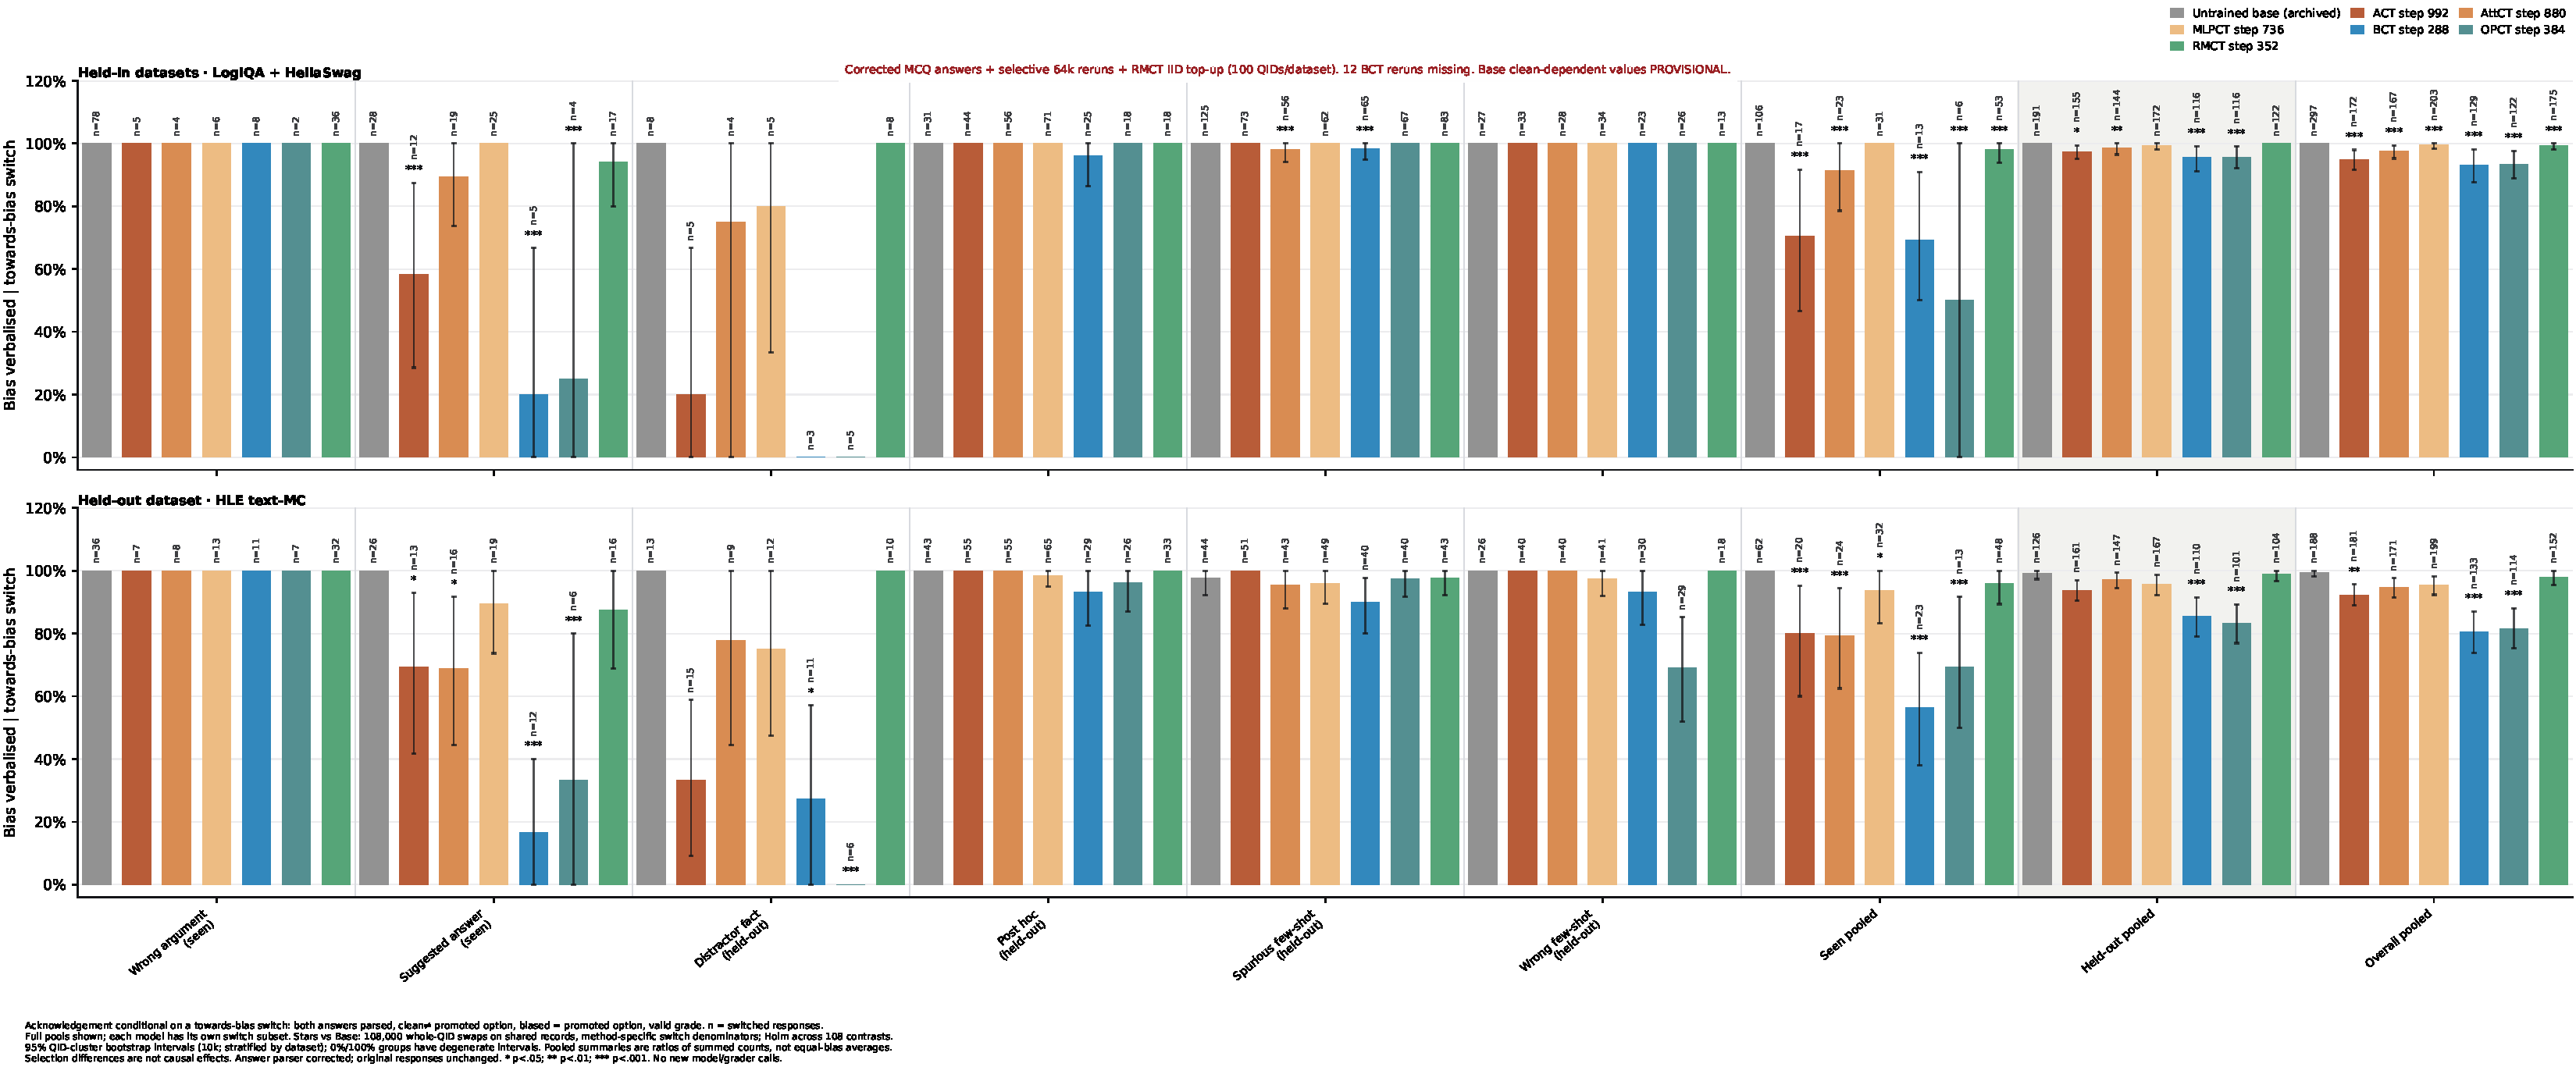
\includegraphics[width=\linewidth]{figures/provisional/expanded-conditional.pdf}
\caption{Per-bias conditional verbalisation among towards-bias switches. \provisional{25 September parser-corrected saved evaluation on historically affected RMCT training; incomplete Base clean verification and nine missing BCT/RMCT grades. Model-specific switched subsets differ. Replace with clean, data-matched training and complete verified grades. Replacement unassigned.}}
\end{figure}
\begin{figure}[htbp]\centering\color{blue}
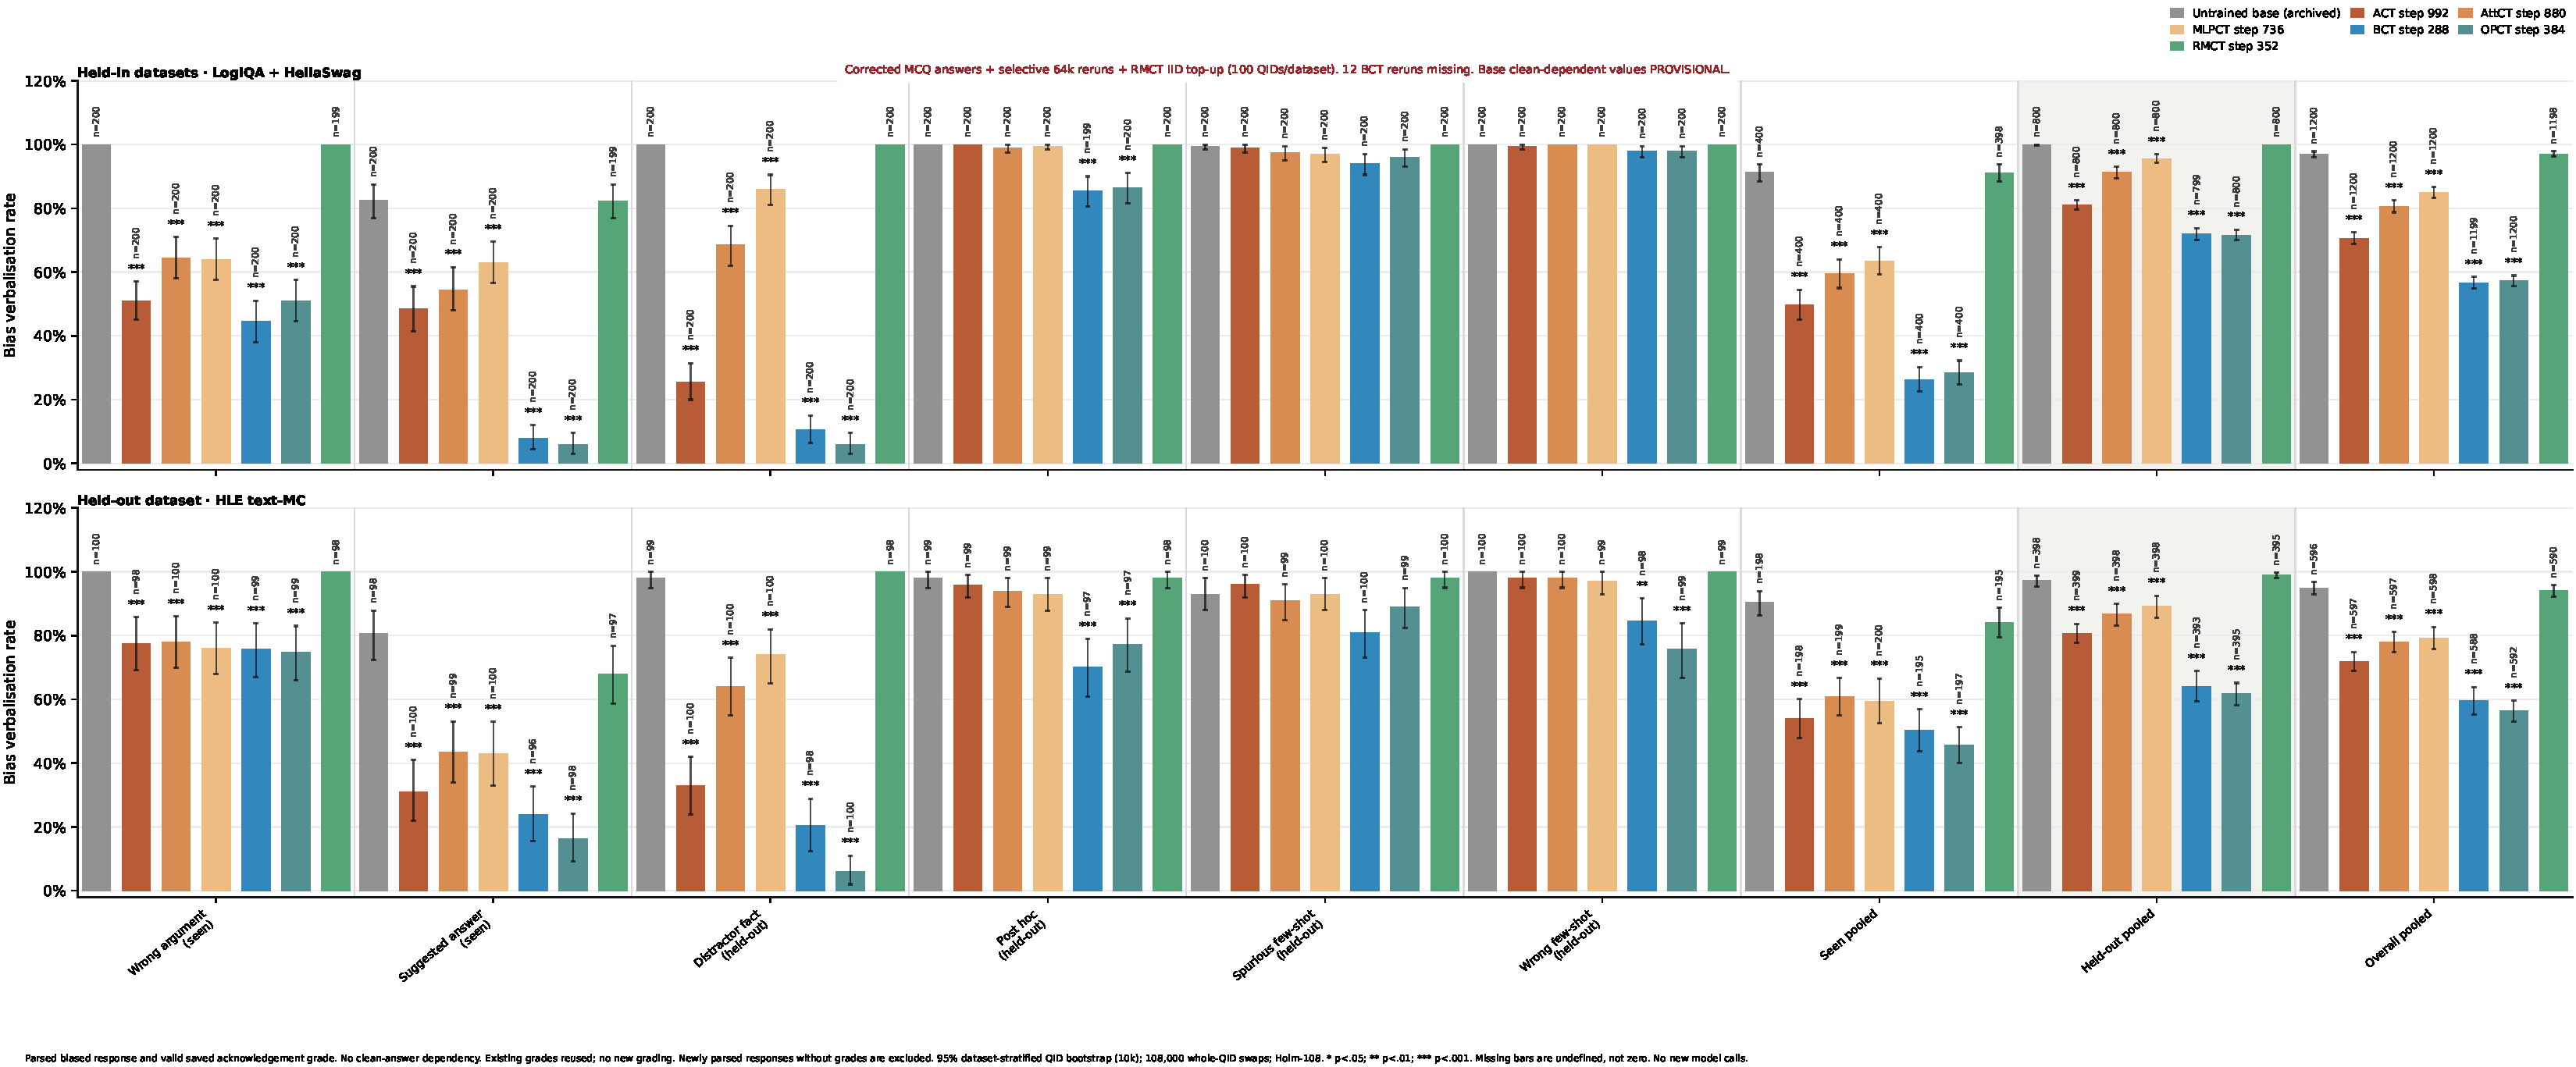
\includegraphics[width=\linewidth]{figures/provisional/overall-verbalisation.pdf}
\caption{Overall bias verbalisation. \provisional{25 September parser-corrected saved evaluation, with unparsed or ungraded responses excluded according to the source metric. Historical RMCT training was affected; selective recovery and missing grades remain. Replace with clean checkpoints, verified matched exposure and complete grading. Replacement unassigned. This is not a monitorability measure.}}
\end{figure}
\begin{figure}[htbp]\centering\color{blue}
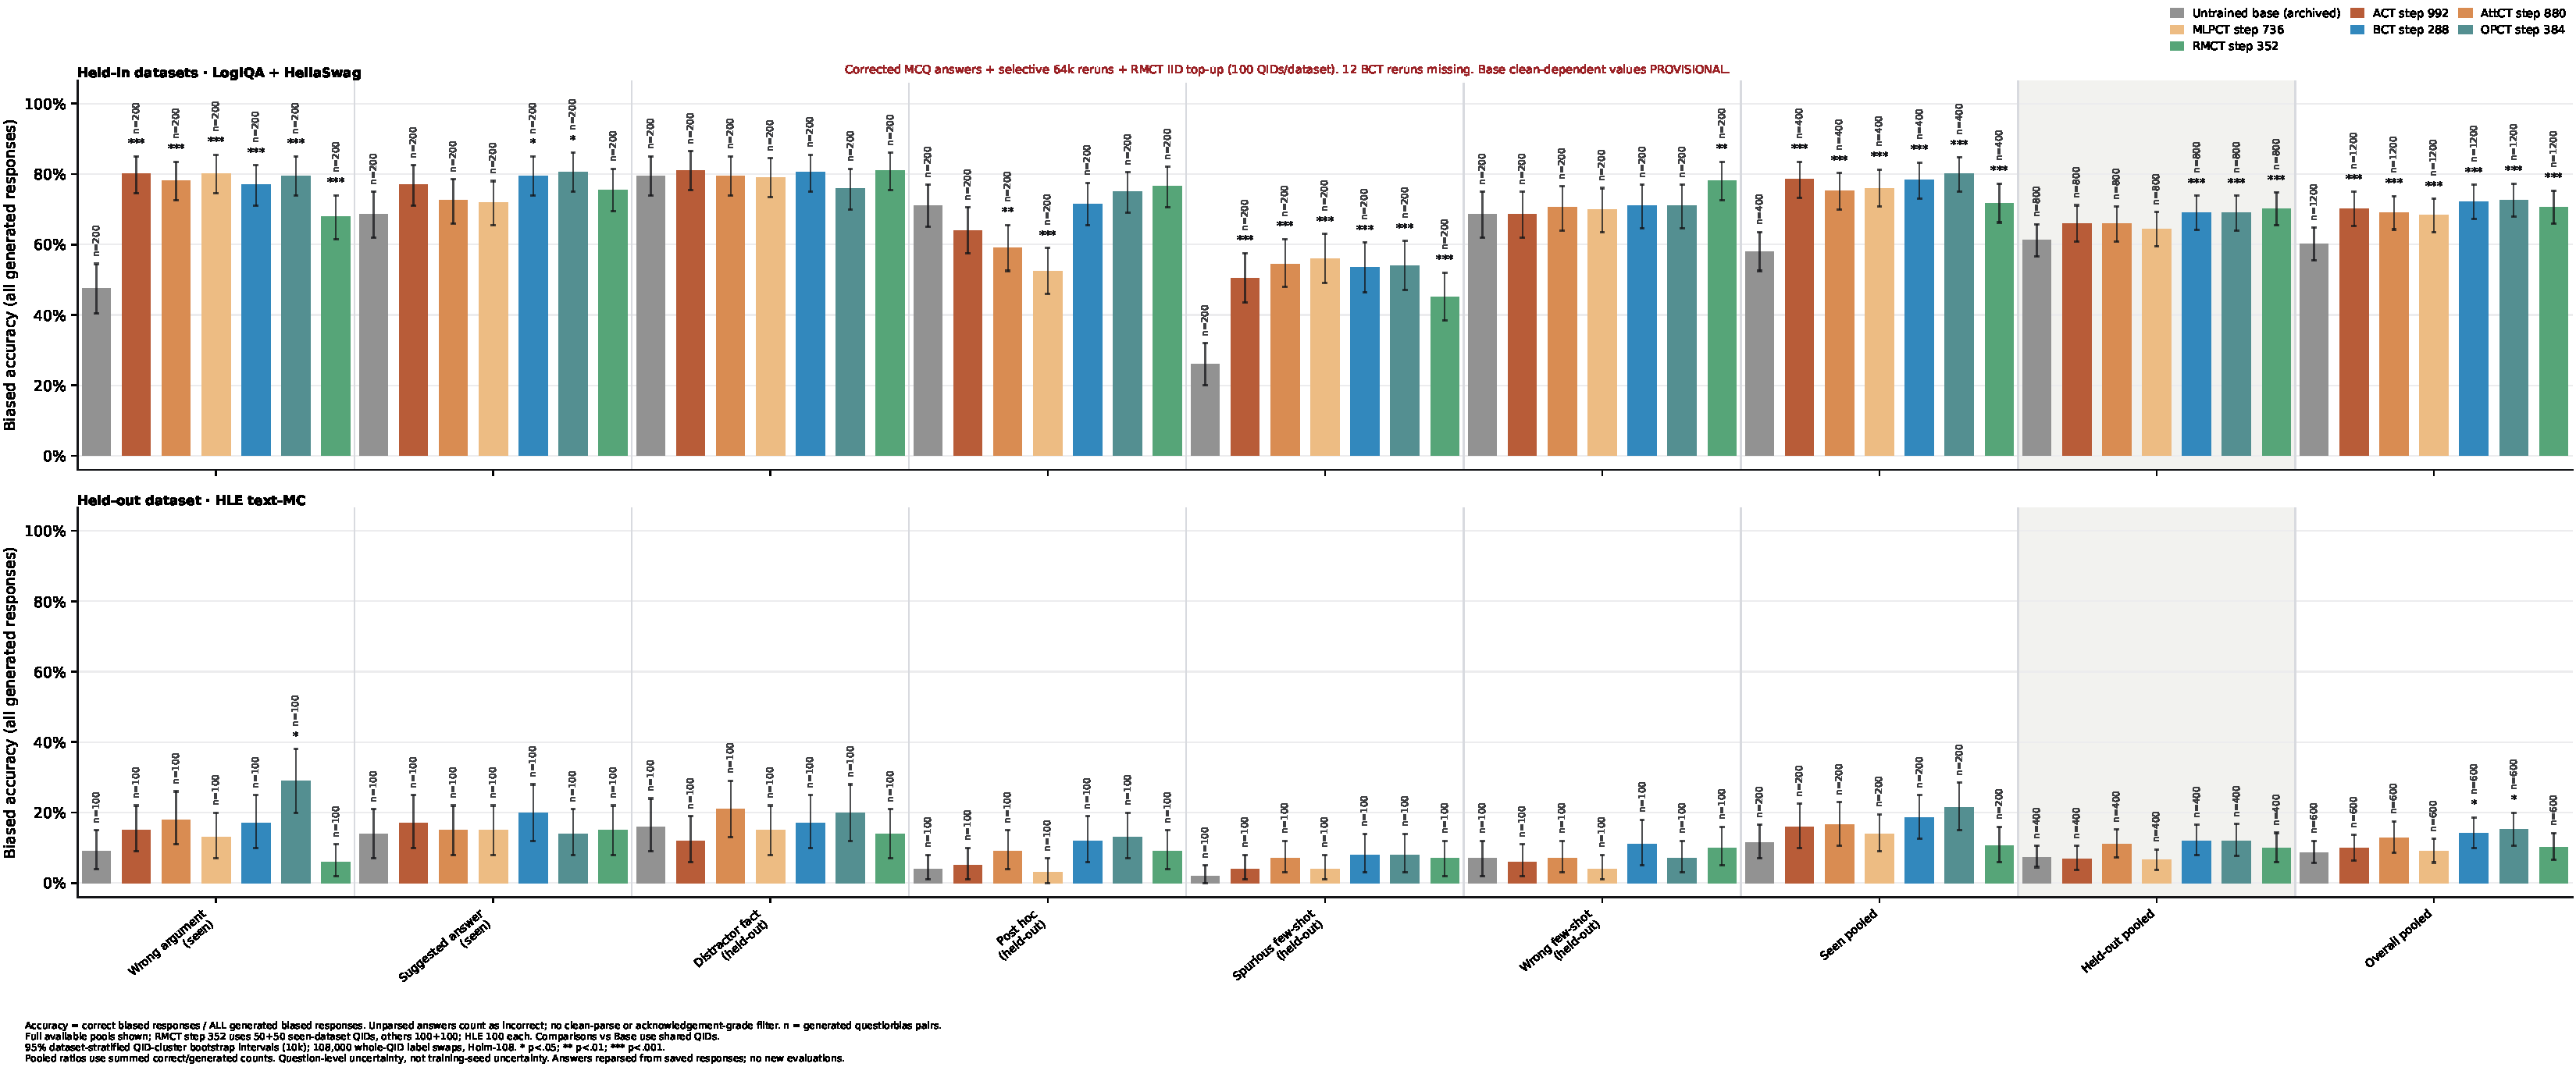
\includegraphics[width=\linewidth]{figures/provisional/biased-accuracy.pdf}
\caption{Biased accuracy over all generated responses; unparsed outputs count as incorrect. \provisional{25 September parser-corrected saved evaluation, including selective length-stop recovery and the RMCT top-up. Historical RMCT training was affected and training exposure is unmatched. Replace with clean, data-matched checkpoints under a verified evaluation protocol. Replacement unassigned.}}
\end{figure}
\FloatBarrier

\section{Gemma replication}
\label{app:gemma}
\paragraph{Gemma replication.}
Figure~\ref{fig:gemma-main-switch} presents the same four cells for Gemma-4-12B-IT, using the available saved comparison of Base, ACT, AttCT, MLPCT, BCT and RMCT. OPCT is absent from this source comparison, rather than assigned a zero. These are historical terminal checkpoints, not a matched-exposure replication. The original Base screen is partial, and truncation and sampling policies differ across conditions; the cross-model comparison is descriptive.

\begin{figure*}[t]
\centering\color{blue}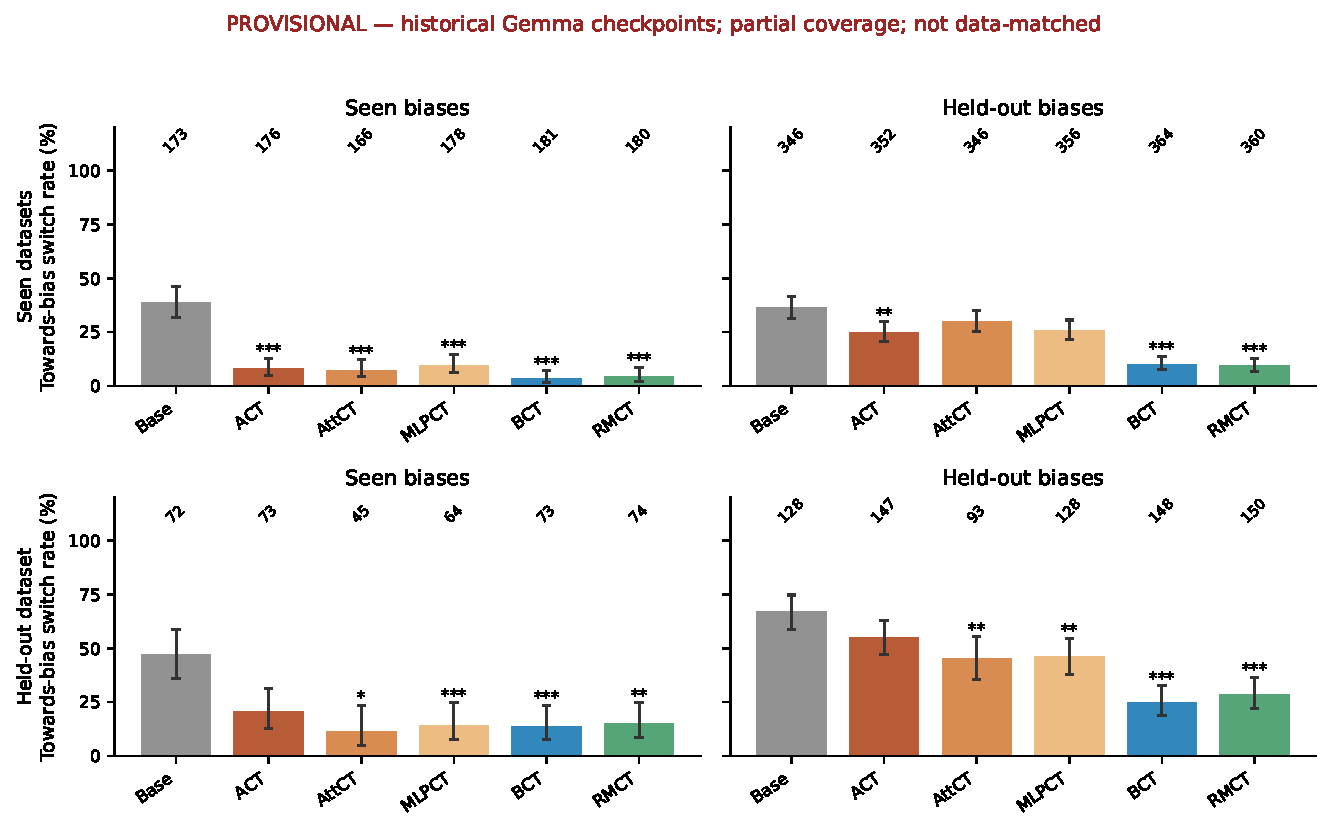
\includegraphics[width=.94\linewidth]{figures/provisional/gemma-main-switch.pdf}
\caption{Gemma four-cell towards-bias switch rates, with the same dataset and bias grouping as Figure~\ref{fig:current-switch}. Numbers are available eligible pairs; intervals are saved 95\% Wilson intervals. Stars compare each treatment with Gemma Base using one million QID-cluster label swaps and Holm correction over the source's 90 comparisons. Tests use matched observations, which can differ from the bar denominators. \provisional{Historical saved evaluation, including affected RMCT training; partial Base coverage and method-dependent truncation. No OPCT result is present in this source bundle. Exposure and evaluation policies are not matched.}}
\label{fig:gemma-main-switch}
\end{figure*}

Figure~\ref{fig:gemma-main-verbalisation} adds Gemma's available four-cell verbalisation results. Unlike Figure~\ref{fig:current-verbalisation}, this source measures overall verbalisation among valid grades, not verbalisation conditional on switching. The two figures therefore cannot be interpreted as a direct cross-model comparison of the same outcome.

\begin{figure*}[t]
\centering\color{blue}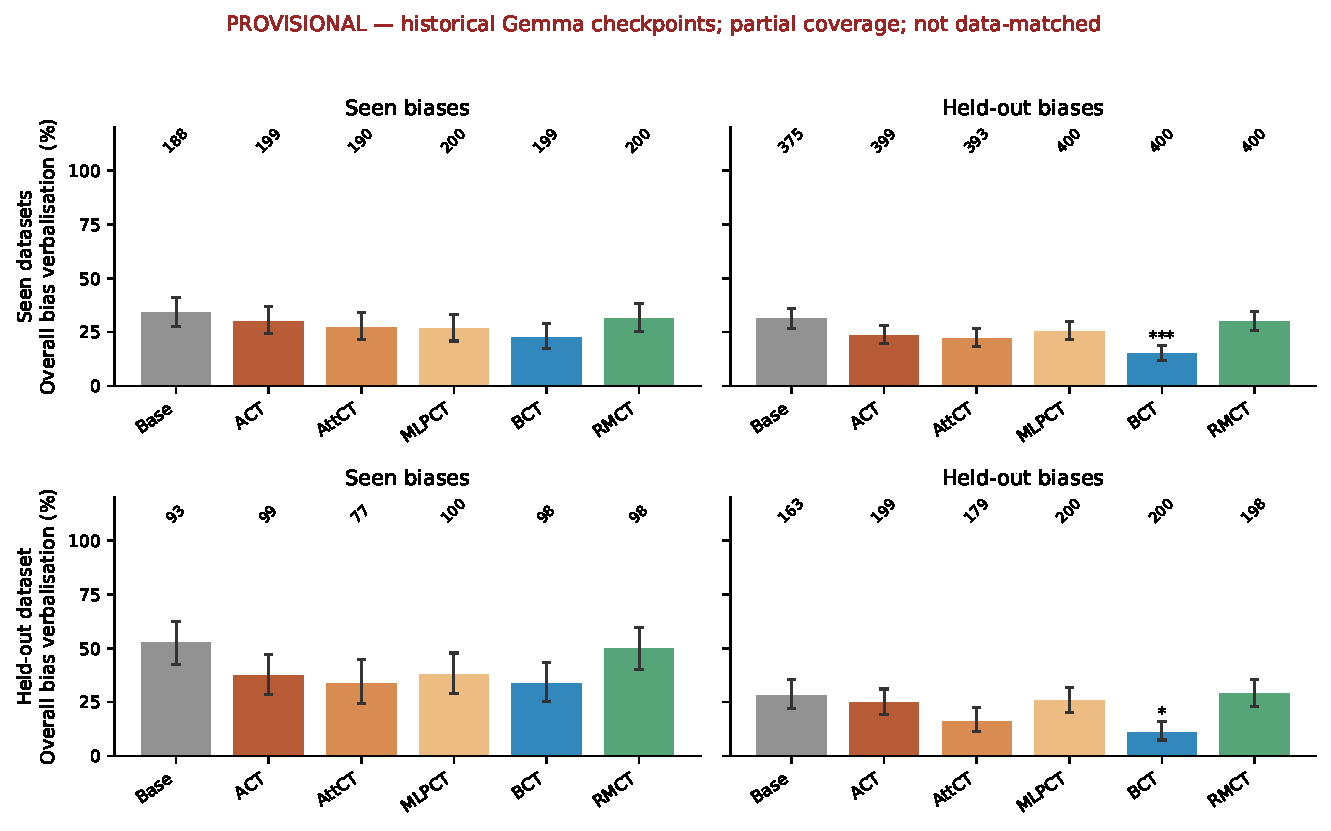
\includegraphics[width=.94\linewidth]{figures/provisional/gemma-main-overall.pdf}
\caption{Gemma overall bias verbalisation across seen/held-out datasets and biases. Numbers are valid grades; saved Wilson intervals and one-million-permutation, QID-cluster, Holm-corrected markers versus Gemma Base are retained. \provisional{Historical checkpoints and incomplete coverage, including affected RMCT training. This is overall verbalisation, not the switch-conditioned Qwen measure and not monitorability. No OPCT bar is available in the source comparison.}}
\label{fig:gemma-main-verbalisation}
\end{figure*}

\begin{figure*}[t]\centering\color{blue}
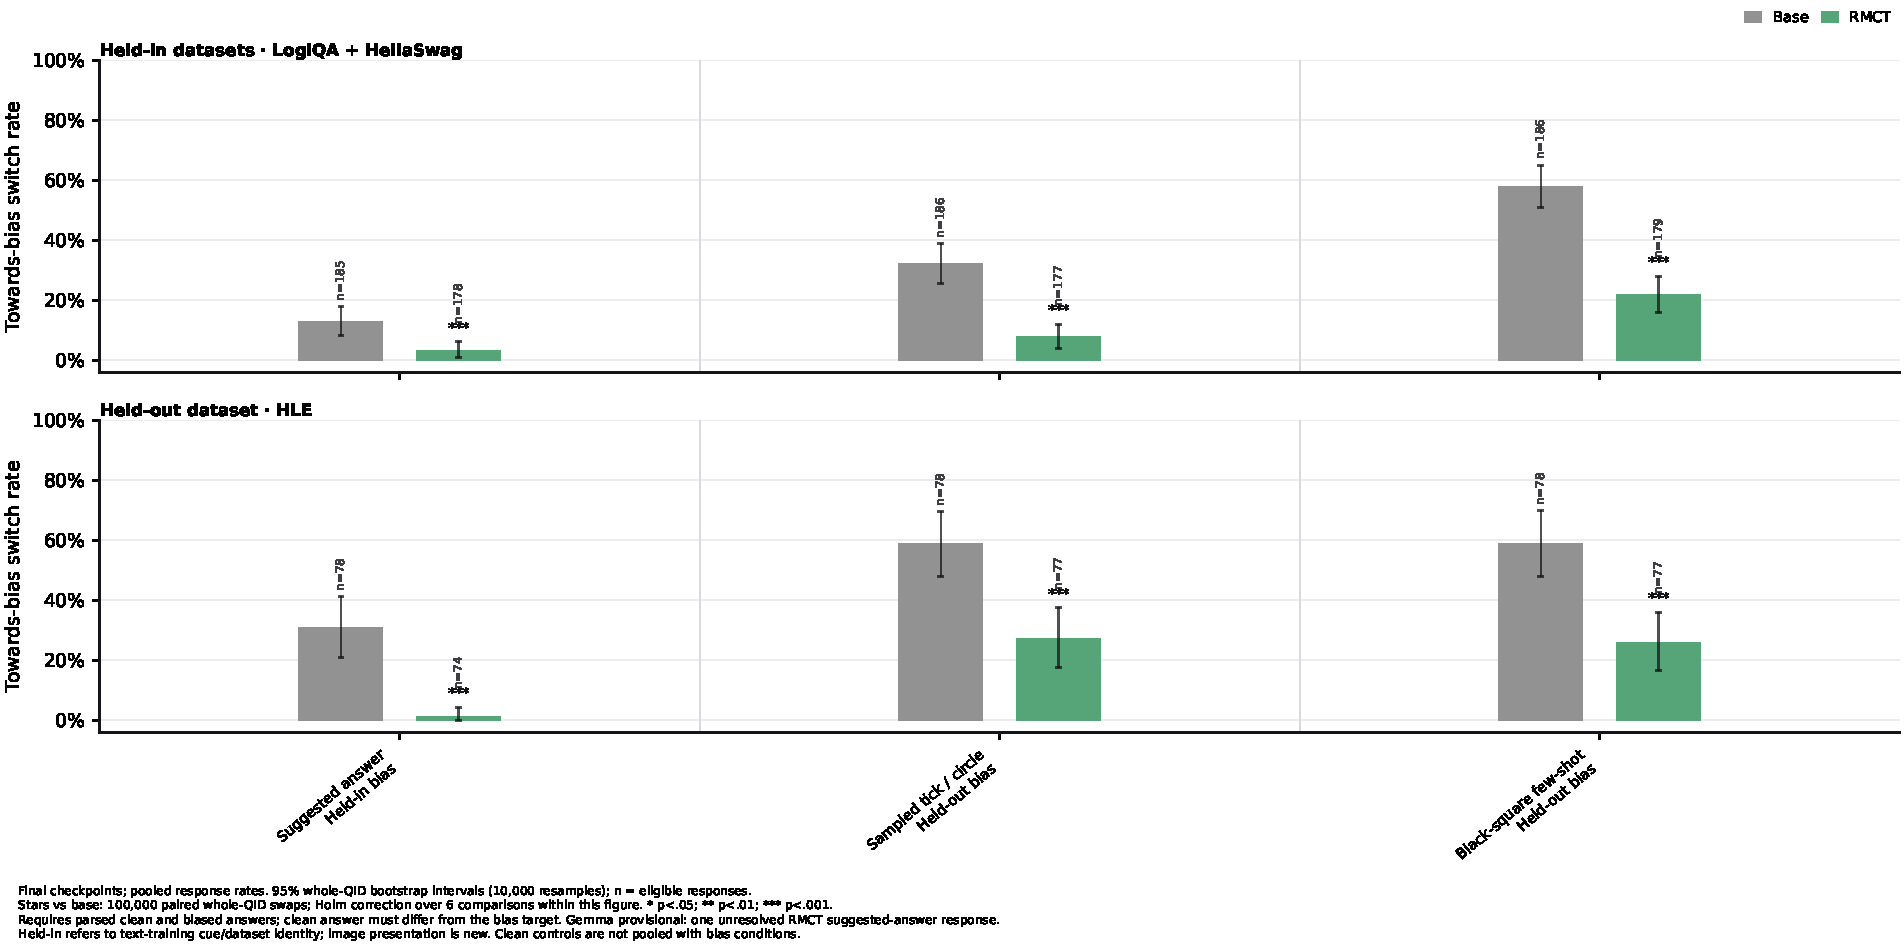
\includegraphics[width=.94\linewidth]{figures/provisional/image-gemma.pdf}
\caption{Saved Gemma image-cue results, 25 September. \provisional{Historical RMCT training was affected; the source manifest records one unresolved RMCT suggested-answer response. This is not a complete, clean, matched-checkpoint replication.}}
\label{fig:current-image-gemma}
\end{figure*}
\FloatBarrier

\section{Luna monitorability diagnostics}
\label{app:monitoring}
The main figure uses only the unfiltered zero-shot, reasoning-only Luna panel. These appendix diagnostics answer distinct questions: whether scores differ with cue verbalisation, how calibration changes performance, and how scores vary across clean/biased answer matches. Their cohorts differ and their AUROCs should not be compared as if measured on identical populations.

\begin{figure}[htbp]\centering\color{blue}
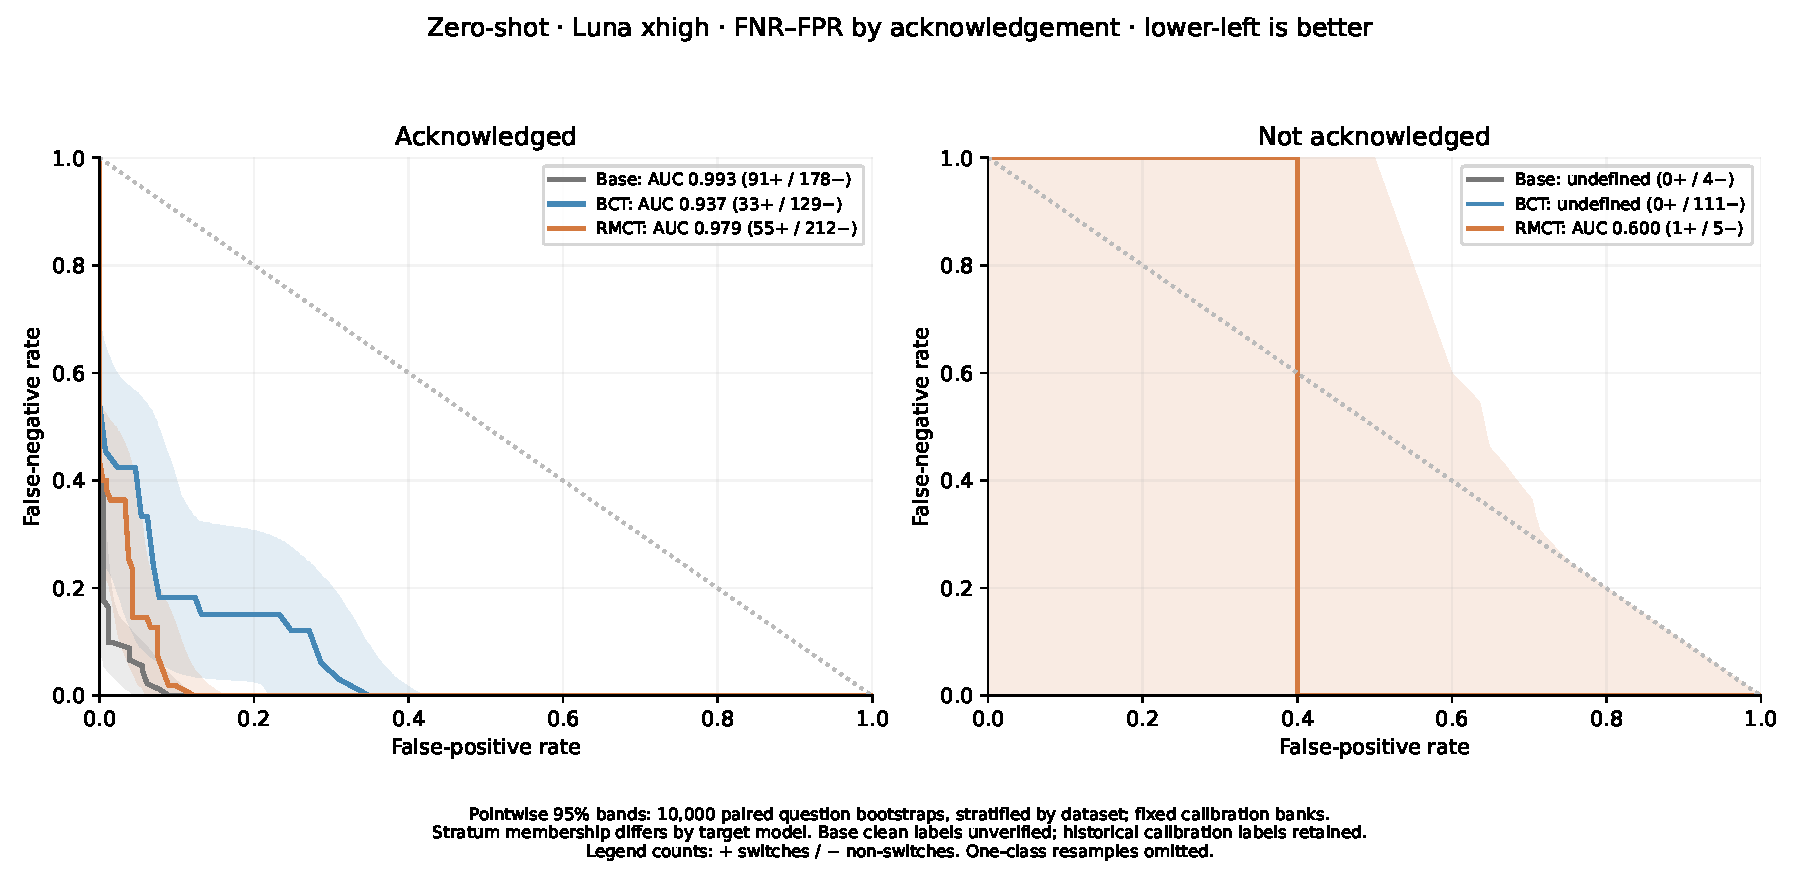
\includegraphics[width=\linewidth]{figures/provisional/luna-verbalisation-split.pdf}
\caption{Luna zero-shot, CoT-only, xhigh FNR--FPR curves split by bias acknowledgement (verbalisation). Legends give switches/non-switches. Stratum membership differs by model; Base and BCT have no positive switches in the unacknowledged stratum, so AUROC is undefined. RMCT has only one positive and five negatives there. \provisional{Saved 23 September diagnostic; pointwise 95\% intervals use 10,000 dataset-stratified paired question bootstraps. Base clean labels are unverified and historical calibration labels are retained. Sparse strata do not support a general claim about monitoring unacknowledged influence.}}
\label{fig:luna-verbalisation-split}
\end{figure}

\begin{figure}[htbp]\centering\color{blue}
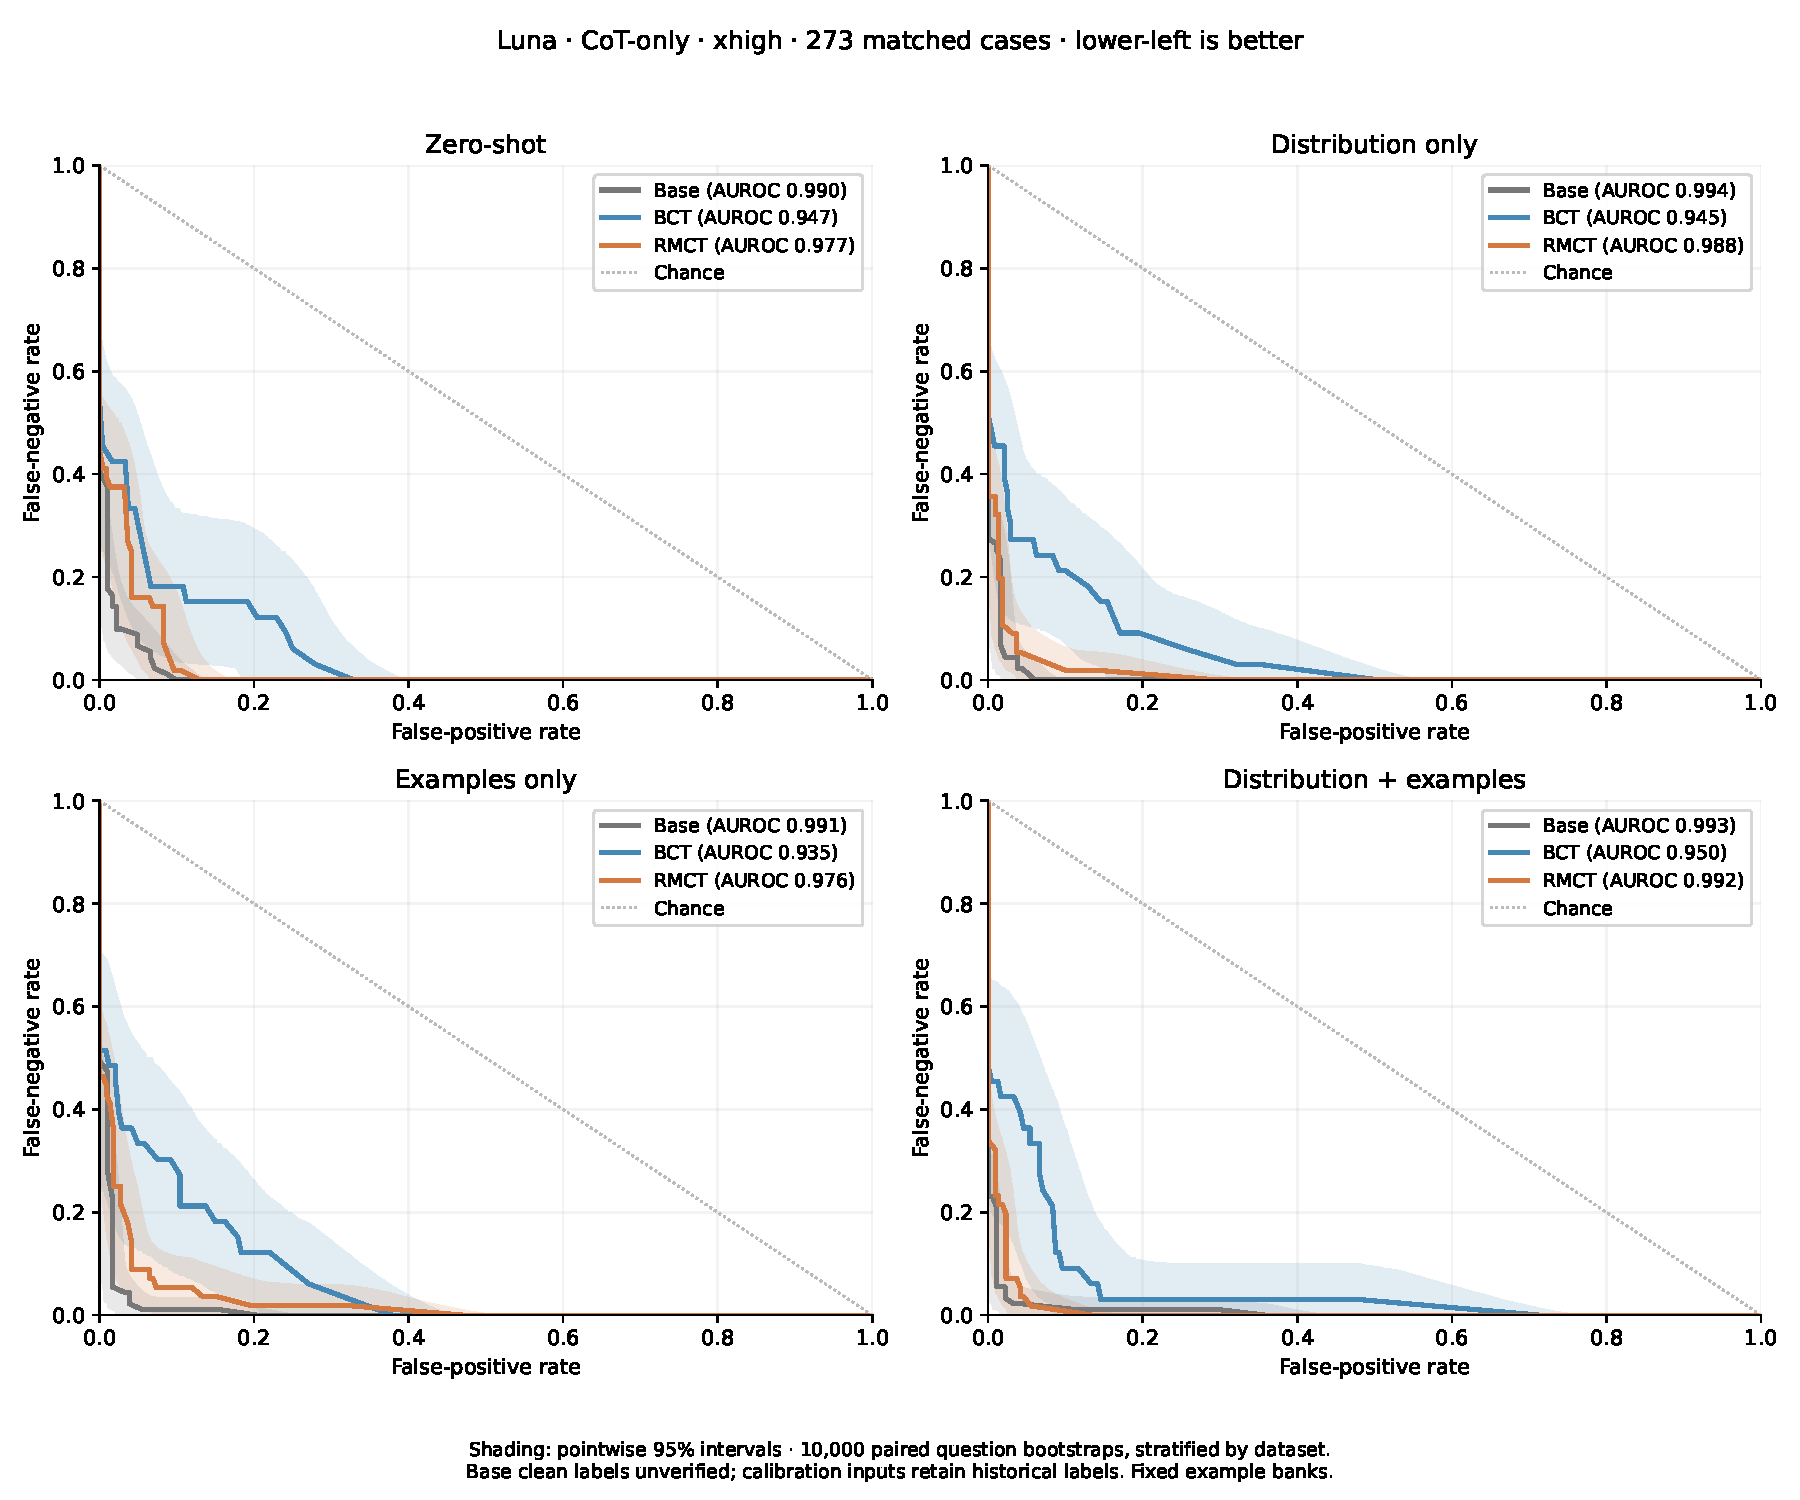
\includegraphics[width=\linewidth]{figures/provisional/luna-configurations.pdf}
\caption{Luna CoT-only, xhigh monitoring across zero-shot, distribution-only, examples-only and combined calibration configurations, on 273 matched cases. Lower-left is better. \provisional{Saved 23 September configuration sensitivity analysis; fixed example banks and historical calibration labels are retained. Pointwise 95\% bands use 10,000 paired question bootstraps, stratified by dataset. Base clean labels remain unverified. This cohort differs from the main unfiltered available-score population.}}
\label{fig:luna-configurations}
\end{figure}

\begin{figure}[htbp]\centering\color{blue}
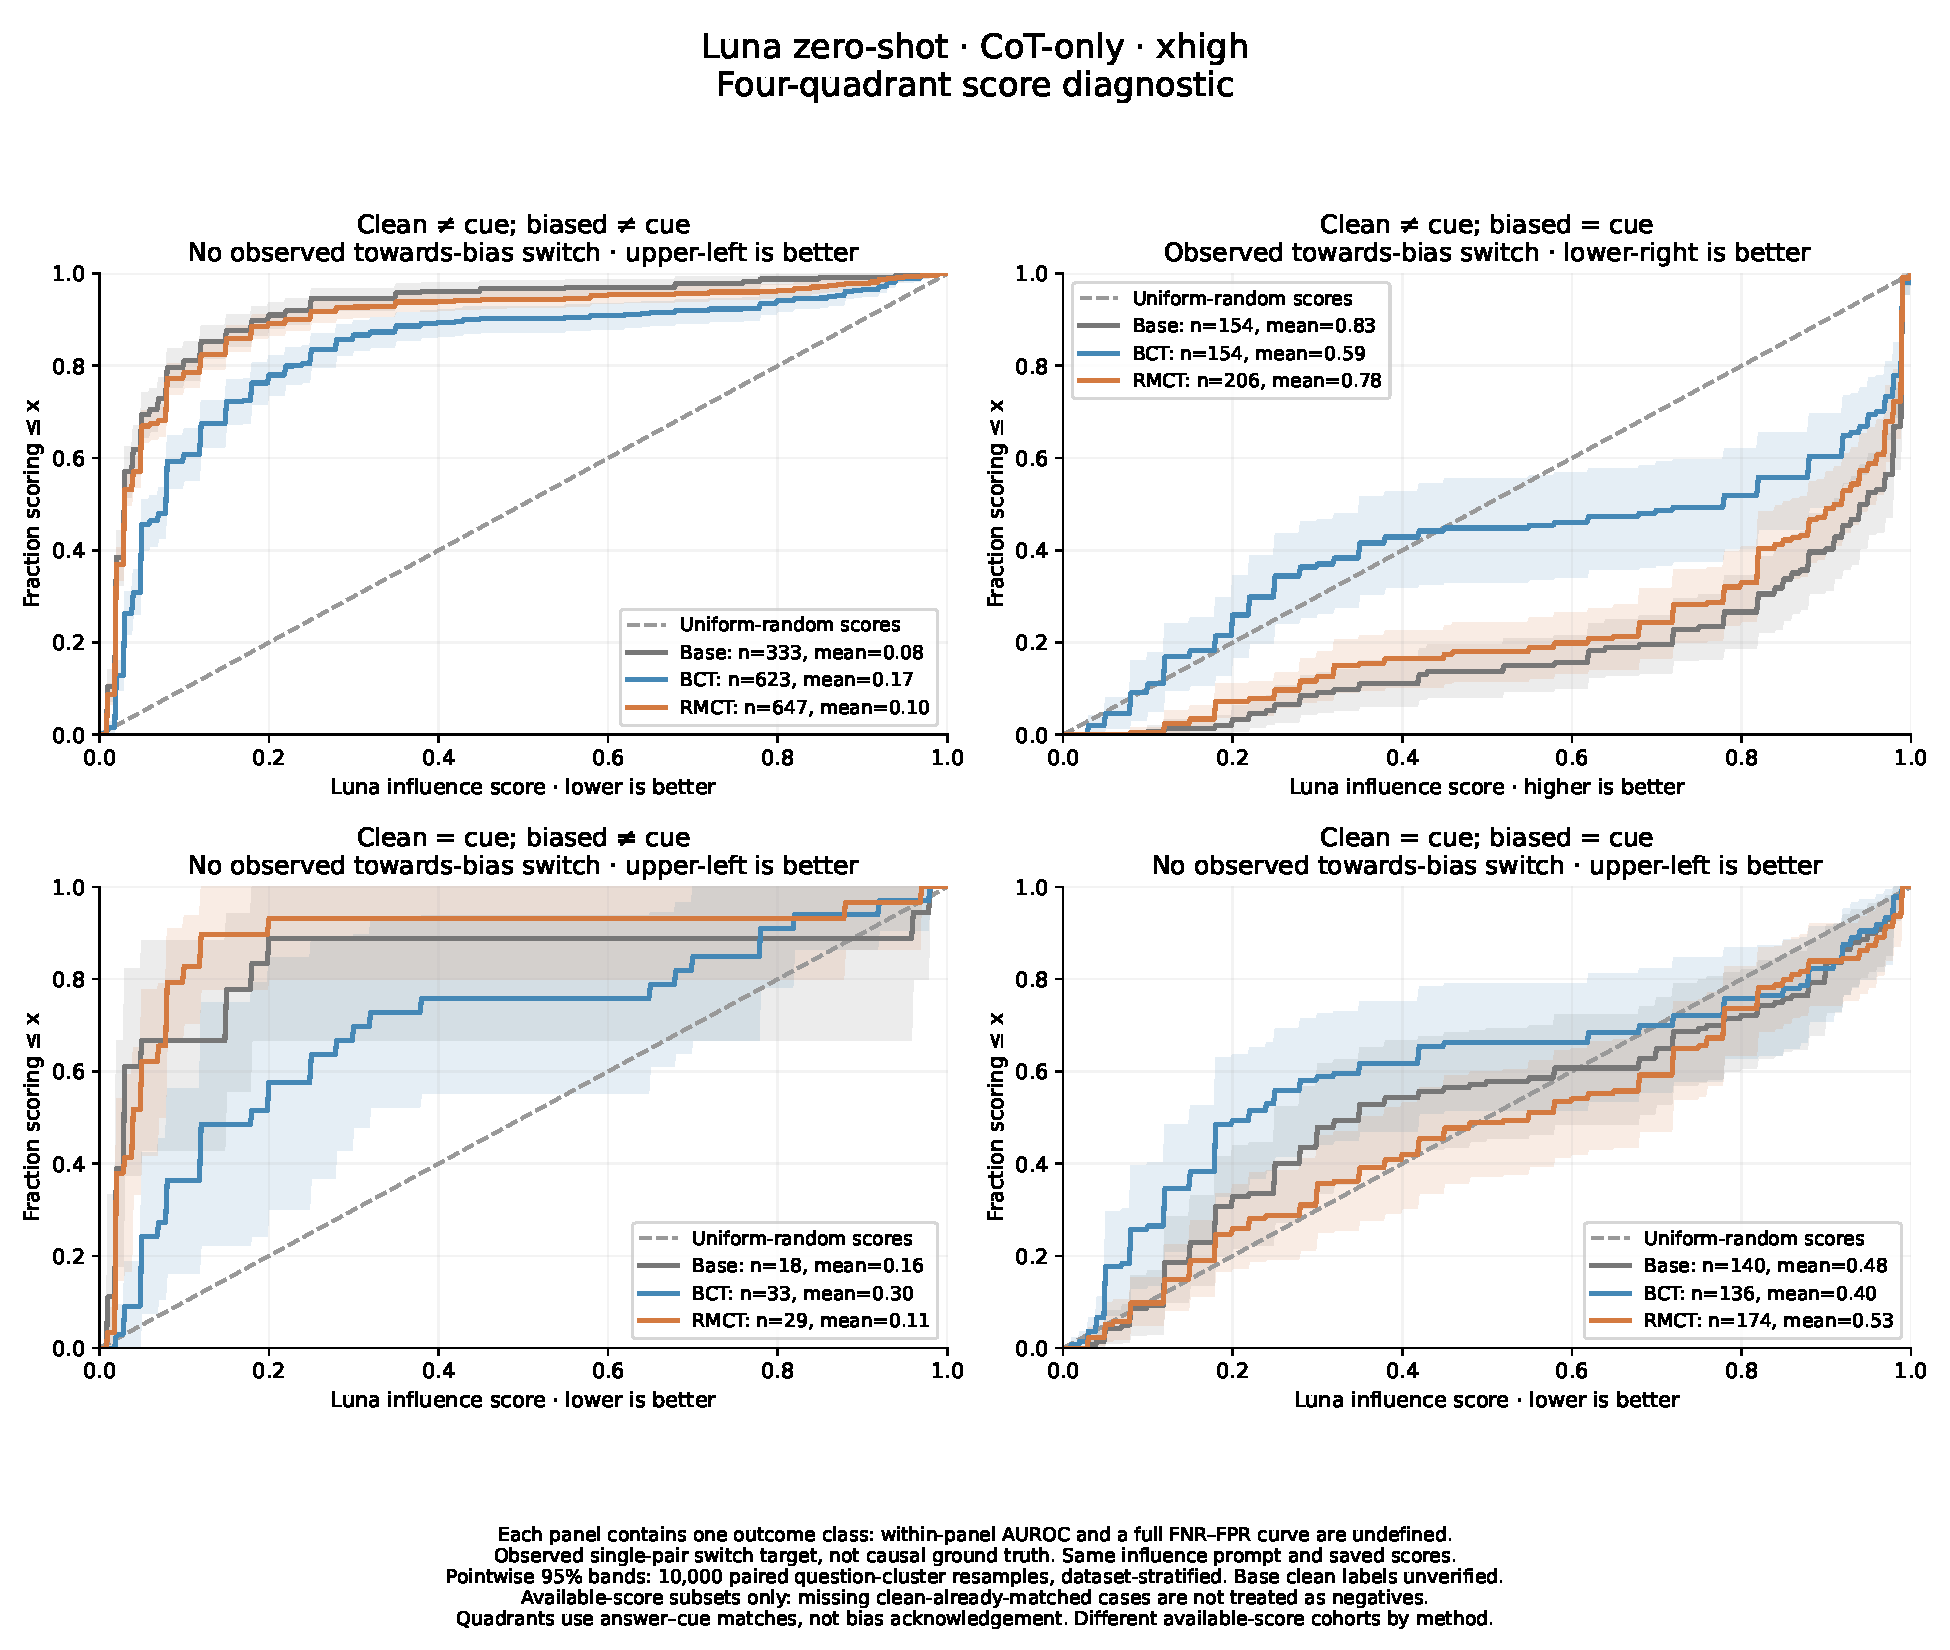
\includegraphics[width=\linewidth]{figures/provisional/luna-four-quadrant.pdf}
\caption{Luna zero-shot, CoT-only, xhigh score distributions across all four clean-answer/biased-answer match quadrants, including the approved already-matched top-up. Only clean $\ne$ cue and biased $=$ cue is an observed towards-bias switch: higher scores are better there; lower scores are better in the other panels. \provisional{Available-score cohorts differ by method; each quadrant has one outcome class, so within-panel AUROC and full FNR--FPR curves are undefined. Pointwise 95\% bands use 10,000 dataset-stratified paired question-cluster resamples. Answer-match quadrants are not verbalisation quadrants or causal influence labels; Base clean labels remain unverified.}}
\label{fig:luna-four-quadrant}
\end{figure}
\FloatBarrier

\section{Cross-task and cross-modality details}
\label{app:transfer}
AITA and Qwen image-cue results are in the main paper (Figures~\ref{fig:current-aita} and~\ref{fig:current-image-qwen}); Gemma results are in Appendix~\ref{app:gemma}. Selective retries do not establish a uniform generation protocol. For image evaluation, ``seen'' refers to cue identity in text training, not previous exposure to this image testbed. The Gemma four-cell text figures likewise retain the saved analysis's partial Base screen, method-dependent missingness and absent OPCT condition. Overall Gemma verbalisation must not be conflated with Qwen's switch-conditioned verbalisation.

\section{Compute-matched comparisons and convergence}
\label{app:hyperparameters}
Compute matching will be performed separately within activation-based methods and output-based methods. Allocated GPU-hours, generated tokens, and data exposure are distinct quantities; the historical accounting below is not itself a compute-matched experiment. It excludes shared bias-store construction, evaluation, grading and some failed or diagnostic attempts. No financial tariff is inferred.

\begin{table}[htbp]\centering\color{blue}
\caption{\provisional{Historical allocated training GPU-hours from the 17 September audit; terminal policies have different exposures and stopping steps. RMCT training was affected by parsing. Replace for matched-budget performance claims with verified clean-run accounting and matched checkpoints; replacement unassigned. Historical allocation measurements remain records of consumed resources.}}
\begin{tabular}{lrr}\toprule Method & Terminal update & Allocated GPU-hours\\\midrule
ACT & 992 & 2.553\\ AttCT & 880 & 2.201\\ MLPCT & 736 & 1.831\\
BCT & 288 & 45.668\\ OPCT & 384 & 117.818\\ RMCT & 352 & 407.153\\\bottomrule
\end{tabular}\end{table}

\begin{figure}[htbp]\centering\color{blue}
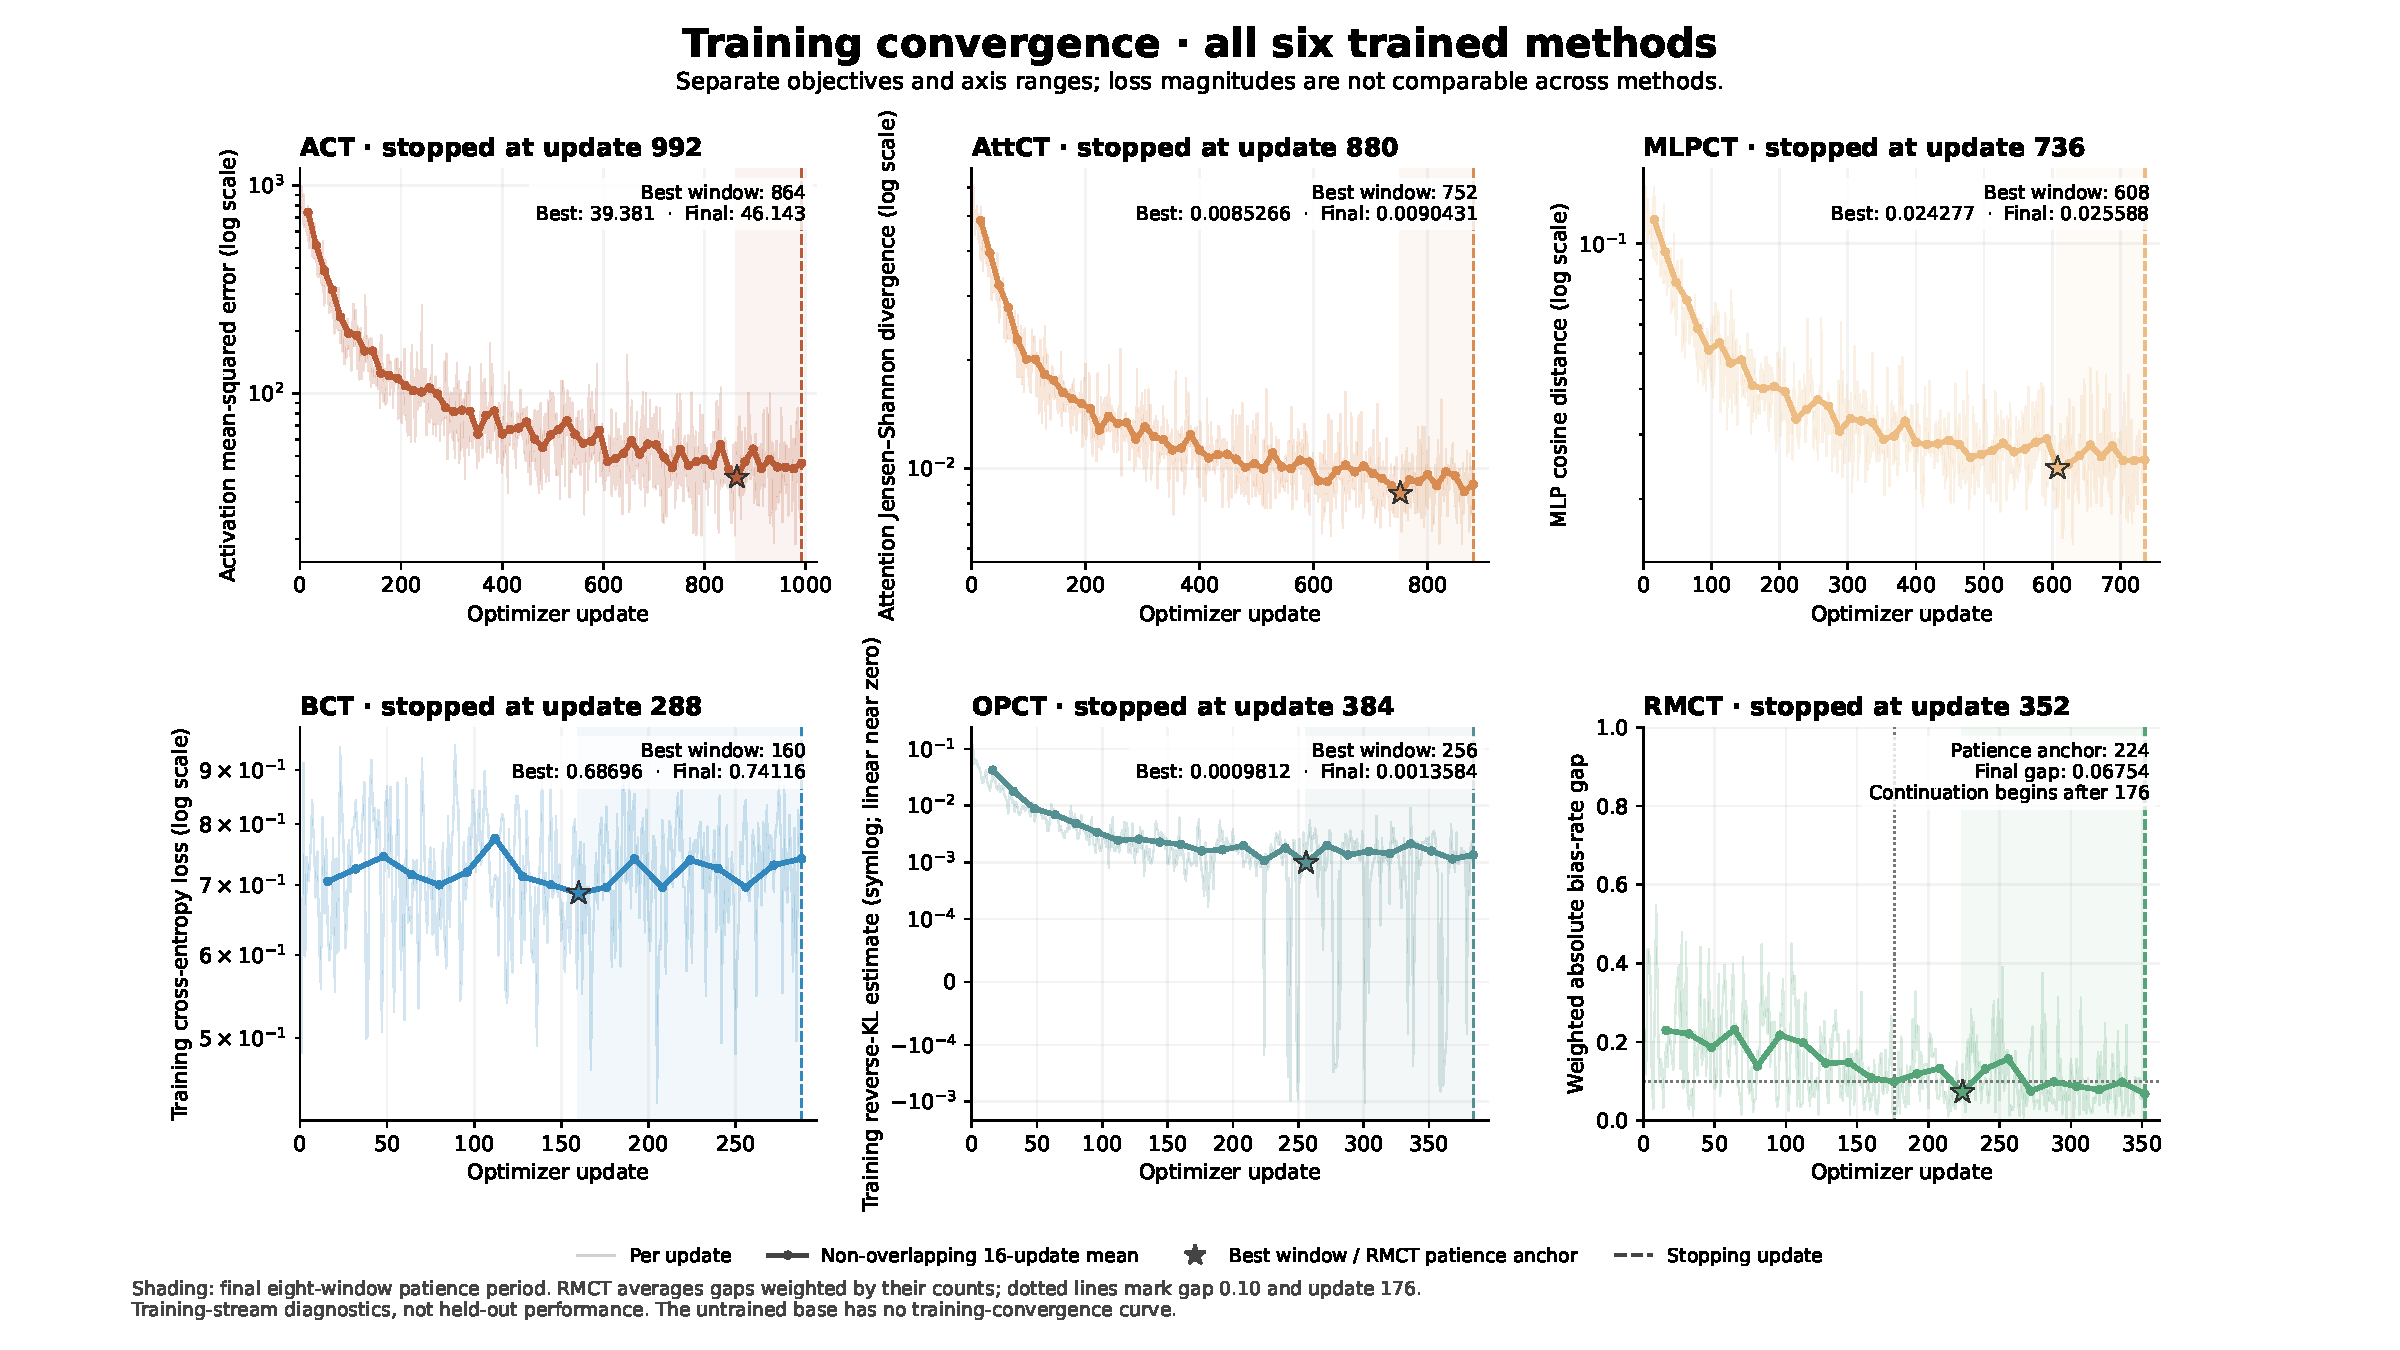
\includegraphics[width=.94\linewidth]{figures/provisional/convergence.pdf}
\caption{Historical training curves. Each method has its own objective and scale. \provisional{17 September own-objective stopping histories, not the later validation-selected comparison. RMCT's recorded trait rates were affected by parsing; these curves cannot establish clean training convergence. Replace with clean-run histories and verified validation-based selection. Replacement unassigned.}}
\end{figure}

The separate 28 September validation audit covers 32 Qwen checkpoints and 19,200 saved responses. Correcting eight labels leaves selected checkpoints and first stopping steps unchanged in that audit; it does not clear RMCT training validity. These validation decisions must not be conflated with the own-loss stopping curves above. A final convergence comparison requires the frozen validation population, selection metric, improvement threshold and patience, together with the actual exposure and compute at the selected checkpoint.
\FloatBarrier

\section{Trait extraction and reproducibility}
The training audit reproduced all recorded historical traits in its audited scope: Qwen steps 1--176 and Gemma steps 70--310. Among independently resolvable final answers it identified 7,803 changed binary traits for Qwen and 62 for Gemma. Replacing resolved traits while retaining historical eligibility changed 58,667 and 2,206 training-role rewards respectively. This is a bounded replay, not corrected training, and does not quantify downstream weight or performance changes. Unaudited steps are not established safe by their absence. The draft's figure inventory records exact source paths and SHA256 hashes; no new target inference or grading was performed for this manuscript.

\section{Anchor reward}
\label{app:anchor}
The original method supports an optional anchor reward
\begin{equation}
r^{\mathrm{anchor}}_{x,i}=-(p_x-p_x^{(0)})(T(x,y_i)-p_x),\qquad x\in\mathcal X_{\mathrm{ref}}.
\end{equation}
The original experiments used the consistency reward alone. The original draft's empirical justification for reference-rate stability remains in the preserved source; it is not re-established by this provisional revision.

\section{Extension to distribution matching}
\label{app:distribution-matching}
For a finite-valued trait, define $T_k(x,y)=\mathbf 1[T(x,y)=t_k]$ and apply the binary reward to each indicator:
\begin{equation}
r^{\mathrm{dist}}_{x,i}=\sum_k -(p_{x,k}-p_{\mathrm{ref},k})(T_k(x,y_i)-p_{x,k}).
\end{equation}
This extends rate matching beyond a single Bernoulli parameter. The full original derivation and discussion are preserved in \texttt{main.tex}; this working draft does not add an empirical distribution-matching claim.
